%        File: arfc-beamer.tex
%     Created: Sun May 5 10:00 PM 2013 C
%


%\documentclass[11pt,handout]{beamer}
\documentclass[9pt]{beamer}
\usetheme[white]{Illinois}
%\title[short title]{long title}
\title[Short Title]{Measurement of Hydrogen $T_1$ and $T_2$ Relaxation Times in Copper Sulfate Solutions Using PNMR}
%\subtitle[short subtitle]{long subtitle}
\subtitle[Short SubTitle]{PNMR Hydrogen Relaxation Times}
%\author[short name]{long name}
\author[Your Name]{Nathan Ryan\\Physics 403, Fall 2021}
%\date[short date]{long date}
\date[09.02.2021]{Oct 12, 2021}
%\institution[short name]{long name}
\institute[UIUC]{University of Illinois at Urbana-Champaign}

%\usepackage{bbding}
\usepackage{amsfonts}
\usepackage{amsmath}
\usepackage{xspace}
\usepackage{graphicx}
\usepackage{subfigure}
\usepackage{booktabs} % nice rules for tables
\usepackage{microtype} % if using PDF
\usepackage{bigints}
\usepackage{minted}
\usepackage{animate}
\usepackage{xmpmulti}


\newcommand{\units}[1] {\:\text{#1}}%
\newcommand{\SN}{S$_N$}%{S$_\text{N}$}%{$S_N$}%
\DeclareMathOperator{\erf}{erf}
%I need some complimentary error funcitons... 
\DeclareMathOperator{\erfc}{erfc}
%Those icons in the references are terrible looking
\setbeamertemplate{bibliography item}[text]

%%%% Acronym support

\usepackage[acronym,toc]{glossaries}
%\newacronym{<++>}{<++>}{<++>}
\newacronym[longplural={metric tons of heavy metal}]{MTHM}{MTHM}{metric ton of heavy metal}
\newacronym{ABM}{ABM}{agent-based modeling}
\newacronym{ACDIS}{ACDIS}{Program in Arms Control \& Domestic and International Security}
\newacronym{AHTR}{AHTR}{Advanced High Temperature Reactor}
\newacronym{ANDRA}{ANDRA}{Agence Nationale pour la gestion des D\'echets RAdioactifs, the French National Agency for Radioactive Waste Management}
\newacronym{ANL}{ANL}{Argonne National Laboratory}
\newacronym{API}{API}{application programming interface}
\newacronym{ARE}{ARE}{Aircraft Reactor Experiment}
\newacronym{ARFC}{ARFC}{Advanced Reactors and Fuel Cycles}
\newacronym{ASME}{ASME}{American Society of Mechanical Engineers}
\newacronym{ATWS}{ATWS}{Anticipated Transient Without Scram}
\newacronym{BDBE}{BDBE}{Beyond Design Basis Event}
\newacronym{BIDS}{BIDS}{Berkeley Institute for Data Science}
\newacronym{CAFCA}{CAFCA}{ Code for Advanced Fuel Cycles Assessment }
\newacronym{CDTN}{CDTN}{Centro de Desenvolvimento da Tecnologia Nuclear}
\newacronym{CEA}{CEA}{Commissariat \`a l'\'Energie Atomique et aux \'Energies Alternatives}
\newacronym{CI}{CI}{continuous integration}
\newacronym{CNEN}{CNEN}{Comiss\~{a}o Nacional de Energia Nuclear}
\newacronym{CNERG}{CNERG}{Computational Nuclear Engineering Research Group}
\newacronym{COSI}{COSI}{Commelini-Sicard}
\newacronym{COTS}{COTS}{commercial, off-the-shelf}
\newacronym{CSNF}{CSNF}{commercial spent nuclear fuel}
\newacronym{CTAH}{CTAHs}{Coiled Tube Air Heaters}
\newacronym{CUBIT}{CUBIT}{CUBIT Geometry and Mesh Generation Toolkit}
\newacronym{CURIE}{CURIE}{Centralized Used Fuel Resource for Information Exchange}
\newacronym{DAG}{DAG}{directed acyclic graph}
\newacronym{DANESS}{DANESS}{Dynamic Analysis of Nuclear Energy System Strategies}
\newacronym{DBE}{DBE}{Design Basis Event}
\newacronym{DESAE}{DESAE}{Dynamic Analysis of Nuclear Energy Systems Strategies}
\newacronym{DHS}{DHS}{Department of Homeland Security}
\newacronym{DOE}{DOE}{Department of Energy}
\newacronym{DRACS}{DRACS}{Direct Reactor Auxiliary Cooling System}
\newacronym{DRE}{DRE}{dynamic resource exchange}
\newacronym{DSNF}{DSNF}{DOE spent nuclear fuel}
\newacronym{DYMOND}{DYMOND}{Dynamic Model of Nuclear Development }
\newacronym{EBS}{EBS}{Engineered Barrier System}
\newacronym{EDZ}{EDZ}{Excavation Disturbed Zone}
\newacronym{EIA}{EIA}{U.S. Energy Information Administration}
\newacronym{EPA}{EPA}{Environmental Protection Agency}
\newacronym{EP}{EP}{Engineering Physics}
\newacronym{FCO}{FCO}{Fuel Cycle Options}
\newacronym{FCT}{FCT}{Fuel Cycle Technology}
\newacronym{FEHM}{FEHM}{Finite Element Heat and Mass Transfer}
\newacronym{FEPs}{FEPs}{Features, Events, and Processes}
\newacronym{FHR}{FHR}{Fluoride-Salt-Cooled High-Temperature Reactor}
\newacronym{FLiBe}{FLiBe}{Fluoride-Lithium-Beryllium}
\newacronym{GDSE}{GDSE}{Generic Disposal System Environment}
\newacronym{GDSM}{GDSM}{Generic Disposal System Model}
\newacronym{GENIUSv1}{GENIUSv1}{Global Evaluation of Nuclear Infrastructure Utilization Scenarios, Version 1}
\newacronym{GENIUSv2}{GENIUSv2}{Global Evaluation of Nuclear Infrastructure Utilization Scenarios, Version 2}
\newacronym{GENIUS}{GENIUS}{Global Evaluation of Nuclear Infrastructure Utilization Scenarios}
\newacronym{GPAM}{GPAM}{Generic Performance Assessment Model}
\newacronym{GRSAC}{GRSAC}{Graphite Reactor Severe Accident Code}
\newacronym{GUI}{GUI}{graphical user interface}
\newacronym{HLW}{HLW}{high level waste}
\newacronym{HPC}{HPC}{high-performance computing}
\newacronym{HTC}{HTC}{high-throughput computing}
\newacronym{HTGR}{HTGR}{High Temperature Gas-Cooled Reactor}
\newacronym{IAEA}{IAEA}{International Atomic Energy Agency}
\newacronym{IEMA}{IEMA}{Illinois Emergency Mangament Agency}
\newacronym{INL}{INL}{Idaho National Laboratory}
\newacronym{IPRR1}{IRP-R1}{Instituto de Pesquisas Radioativas Reator 1}
\newacronym{IRP}{IRP}{Integrated Research Project}
\newacronym{ISFSI}{ISFSI}{Independent Spent Fuel Storage Installation}
\newacronym{ISRG}{ISRG}{Independent Student Research Group}
\newacronym{JFNK}{JFNK}{Jacobian-Free Newton Krylov}
\newacronym{LANL}{LANL}{Los Alamos National Laboratory}
\newacronym{LBNL}{LBNL}{Lawrence Berkeley National Laboratory}
\newacronym{LCOE}{LCOE}{levelized cost of electricity}
\newacronym{LDRD}{LDRD}{laboratory directed research and development}
\newacronym{LFR}{LFR}{Lead-Cooled Fast Reactor}
\newacronym{LLNL}{LLNL}{Lawrence Livermore National Laboratory}
\newacronym{LMFBR}{LMFBR}{Liquid Metal Fast Breeder Reactor}
\newacronym{LOFC}{LOFC}{Loss of Forced Cooling}
\newacronym{LOHS}{LOHS}{Loss of Heat Sink}
\newacronym{LOLA}{LOLA}{Loss of Large Area}
\newacronym{LP}{LP}{linear program}
\newacronym{MA}{MA}{minor actinide}
\newacronym{MCNP}{MCNP}{Monte Carlo N-Particle code}
\newacronym{MILP}{MILP}{mixed-integer linear program}
\newacronym{MIT}{MIT}{the Massachusetts Institute of Technology}
\newacronym{MOAB}{MOAB}{Mesh-Oriented datABase}
\newacronym{MOOSE}{MOOSE}{Multiphysics Object-Oriented Simulation Environment}
\newacronym{MOX}{MOX}{mixed oxide}
\newacronym{MSBR}{MSBR}{Molten Salt Breeder Reactor}
\newacronym{MSRE}{MSRE}{Molten Salt Reactor Experiment}
\newacronym{MSR}{MSR}{Molten Salt Reactor}
\newacronym{NAGRA}{NAGRA}{National Cooperative for the Disposal of Radioactive Waste}
\newacronym{NEAMS}{NEAMS}{Nuclear Engineering Advanced Modeling and Simulation}
\newacronym{NEUP}{NEUP}{Nuclear Energy University Programs}
\newacronym{NFCSim}{NFCSim}{Nuclear Fuel Cycle Simulator}
\newacronym{NGNP}{NGNP}{Next Generation Nuclear Plant}
\newacronym{NMWPC}{NMWPC}{Nuclear MW Per Capita}
\newacronym{NNSA}{NNSA}{National Nuclear Security Administration}
\newacronym{NPRE}{NPRE}{Department of Nuclear, Plasma, and Radiological Engineering}
\newacronym{NQA1}{NQA-1}{Nuclear Quality Assurance - 1}
\newacronym{NRC}{NRC}{Nuclear Regulatory Commission}
\newacronym{NSF}{NSF}{National Science Foundation}
\newacronym{NSSC}{NSSC}{Nuclear Science and Security Consortium}
\newacronym{NUWASTE}{NUWASTE}{Nuclear Waste Assessment System for Technical Evaluation}
\newacronym{NWF}{NWF}{Nuclear Waste Fund}
\newacronym{NWTRB}{NWTRB}{Nuclear Waste Technical Review Board}
\newacronym{OCRWM}{OCRWM}{Office of Civilian Radioactive Waste Management}
\newacronym{ORION}{ORION}{ORION}
\newacronym{ORNL}{ORNL}{Oak Ridge National Laboratory}
\newacronym{PARCS}{PARCS}{Purdue Advanced Reactor Core Simulator}
\newacronym{PBAHTR}{PB-AHTR}{Pebble Bed Advanced High Temperature Reactor}
\newacronym{PBFHR}{PB-FHR}{Pebble-Bed Fluoride-Salt-Cooled High-Temperature Reactor}
\newacronym{PEI}{PEI}{Peak Environmental Impact}
\newacronym{PH}{PRONGHORN}{PRONGHORN}
\newacronym{PRKE}{PRKE}{Point Reactor Kinetics Equations}
\newacronym{PSPG}{PSPG}{Pressure-Stabilizing/Petrov-Galerkin}
\newacronym{PWAR}{PWAR}{Pratt and Whitney Aircraft Reactor}
\newacronym{PWR}{PWR}{Pressurized Water Reactor}
\newacronym{PyNE}{PyNE}{Python toolkit for Nuclear Engineering}
\newacronym{PyRK}{PyRK}{Python for Reactor Kinetics}
\newacronym{QA}{QA}{quality assurance}
\newacronym{RDD}{RD\&D}{Research Development and Demonstration}
\newacronym{RD}{R\&D}{Research and Development}
\newacronym{RELAP}{RELAP}{Reactor Excursion and Leak Analysis Program}
\newacronym{RIA}{RIA}{Reactivity Insertion Accident}
\newacronym{RIF}{RIF}{Region-Institution-Facility}
\newacronym{SFR}{SFR}{Sodium-Cooled Fast Reactor}
\newacronym{SINDAG}{SINDA{\textbackslash}G}{Systems Improved Numerical Differencing Analyzer $\backslash$ Gaski}
\newacronym{SKB}{SKB}{Svensk K\"{a}rnbr\"{a}nslehantering AB}
\newacronym{SNF}{SNF}{spent nuclear fuel}
\newacronym{SNL}{SNL}{Sandia National Laboratory}
\newacronym{STC}{STC}{specific temperature change}
\newacronym{SUPG}{SUPG}{Streamline-Upwind/Petrov-Galerkin}
\newacronym{SWF}{SWF}{Separations and Waste Forms}
\newacronym{SWU}{SWU}{Separative Work Unit}
\newacronym{TRIGA}{TRIGA}{Training Research Isotope General Atomic}
\newacronym{TRISO}{TRISO}{Tristructural Isotropic}
\newacronym{TSM}{TSM}{Total System Model}
\newacronym{TSPA}{TSPA}{Total System Performance Assessment for the Yucca Mountain License Application}
\newacronym{ThOX}{ThOX}{thorium oxide}
\newacronym{UFD}{UFD}{Used Fuel Disposition}
\newacronym{UML}{UML}{Unified Modeling Language}
\newacronym{UOX}{UOX}{uranium oxide}
\newacronym{UQ}{UQ}{uncertainty quantification}
\newacronym{US}{US}{United States}
\newacronym{UW}{UW}{University of Wisconsin}
\newacronym{VISION}{VISION}{the Verifiable Fuel Cycle Simulation Model}
\newacronym{VV}{V\&V}{verification and validation}
\newacronym{WIPP}{WIPP}{Waste Isolation Pilot Plant}
\newacronym{YMR}{YMR}{Yucca Mountain Repository Site}


\makeglossaries

%try to get rid of header on title page\dots
\makeatletter
    \newenvironment{withoutheadline}{
        \setbeamertemplate{headline}[default]
        \def\beamer@entrycode{\vspace*{-\headheight}}
    }{}
\makeatother

\makeatother
\setbeamertemplate{footline}
{
  \leavevmode%
  \hbox{%
    \rightline{\insertframenumber{} / \inserttotalframenumber\hspace*{1ex}}
  }%
  \vskip0pt%
}
\makeatletter
\begin{document}
%%%%%%%%%%%%%%%%%%%%%%%%%%%%%%%%%%%%%%%%%%%%%%%%%%%%%%%%%%%%%
%% From uw-beamer Here's a handy bit of code to place at 
%% the beginning of your presentation (after \begin{document}):
\newcommand*{\alphabet}{ABCDEFGHIJKLMNOPQRSTUVWXYZabcdefghijklmnopqrstuvwxyz}
\newlength{\highlightheight}
\newlength{\highlightdepth}
\newlength{\highlightmargin}
\setlength{\highlightmargin}{2pt}
\settoheight{\highlightheight}{\alphabet}
\settodepth{\highlightdepth}{\alphabet}
\addtolength{\highlightheight}{\highlightmargin}
\addtolength{\highlightdepth}{\highlightmargin}
\addtolength{\highlightheight}{\highlightdepth}
\newcommand*{\Highlight}{\rlap{\textcolor{HighlightBackground}{\rule[-\highlightdepth]{\linewidth}{\highlightheight}}}}
%%%%%%%%%%%%%%%%%%%%%%%%%%%%%%%%%%%%%%%%%%%%%%%%%%%%%%%%%%%%%
%%--------------------------------%%
\begin{withoutheadline}
\frame{
  \titlepage
}
\end{withoutheadline}

%%--------------------------------%%
\AtBeginSection[]{
\begin{frame}
  \frametitle{Outline}
  \tableofcontents[currentsection]
\end{frame}
}

\section{Background}
\subsection{Theory}
\begin{frame}[fragile]
  \frametitle{What is PNMR?}
  PNMR, or Pulsed Nuclear Magnetic Resonance, falls under the umbrella of MRI techniques that many of us are familiar with. 
  \begin{figure}
  \begin{center}
        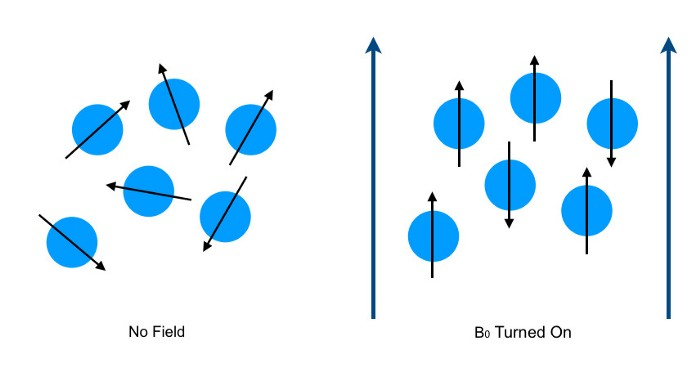
\includegraphics[height=5cm]{./images/polarization.jpeg}
\end{center}
\caption{Initial Polarization \cite{init_polar}}
\label{fig:relax}
\end{figure}
\end{frame}

\begin{frame}
  \frametitle{Relaxation Path}
  % a comment
  \begin{figure}[htbp!]
    \begin{center}
      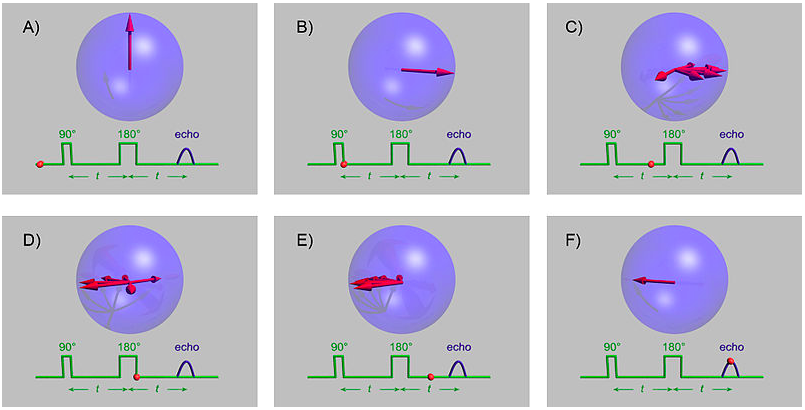
\includegraphics[height=5.2cm]{./images/figures/theory/relax.png}
    \end{center}
          \caption{General Relaxation Path \cite{spin_echo}}
    \label{fig:relax}
  \end{figure}
\end{frame}

\begin{frame}
  \frametitle{Relaxation Path}
  \begin{figure}
  \begin{center}
    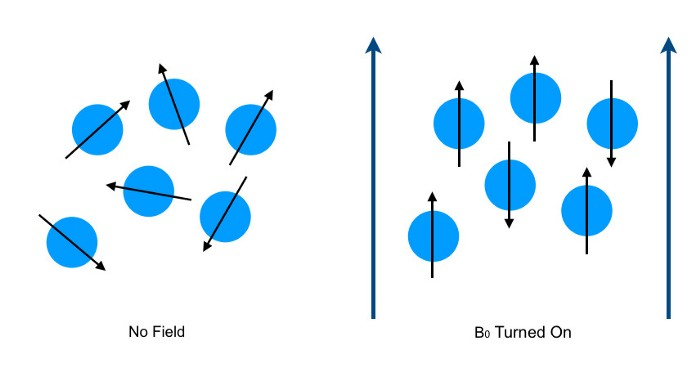
\includegraphics[height=5cm]{./images/polarization.jpeg}
  \end{center}
    \caption{\cite{spin_echo}}
    \label{fig:animate}
\end{figure}
\end{frame}

\subsection{Goal and Motivation}
\begin{frame}
  \frametitle{Goal and Motivation}
  % a comment
        \begin{columns}
                \column[t]{5cm}
                \vspace{25mm}
                

                Characterize the relationship between relaxation time of hydrogen and concentration of a solute.
                \column[t]{5cm}
        \begin{figure}[htbp!]
        \begin{center}
      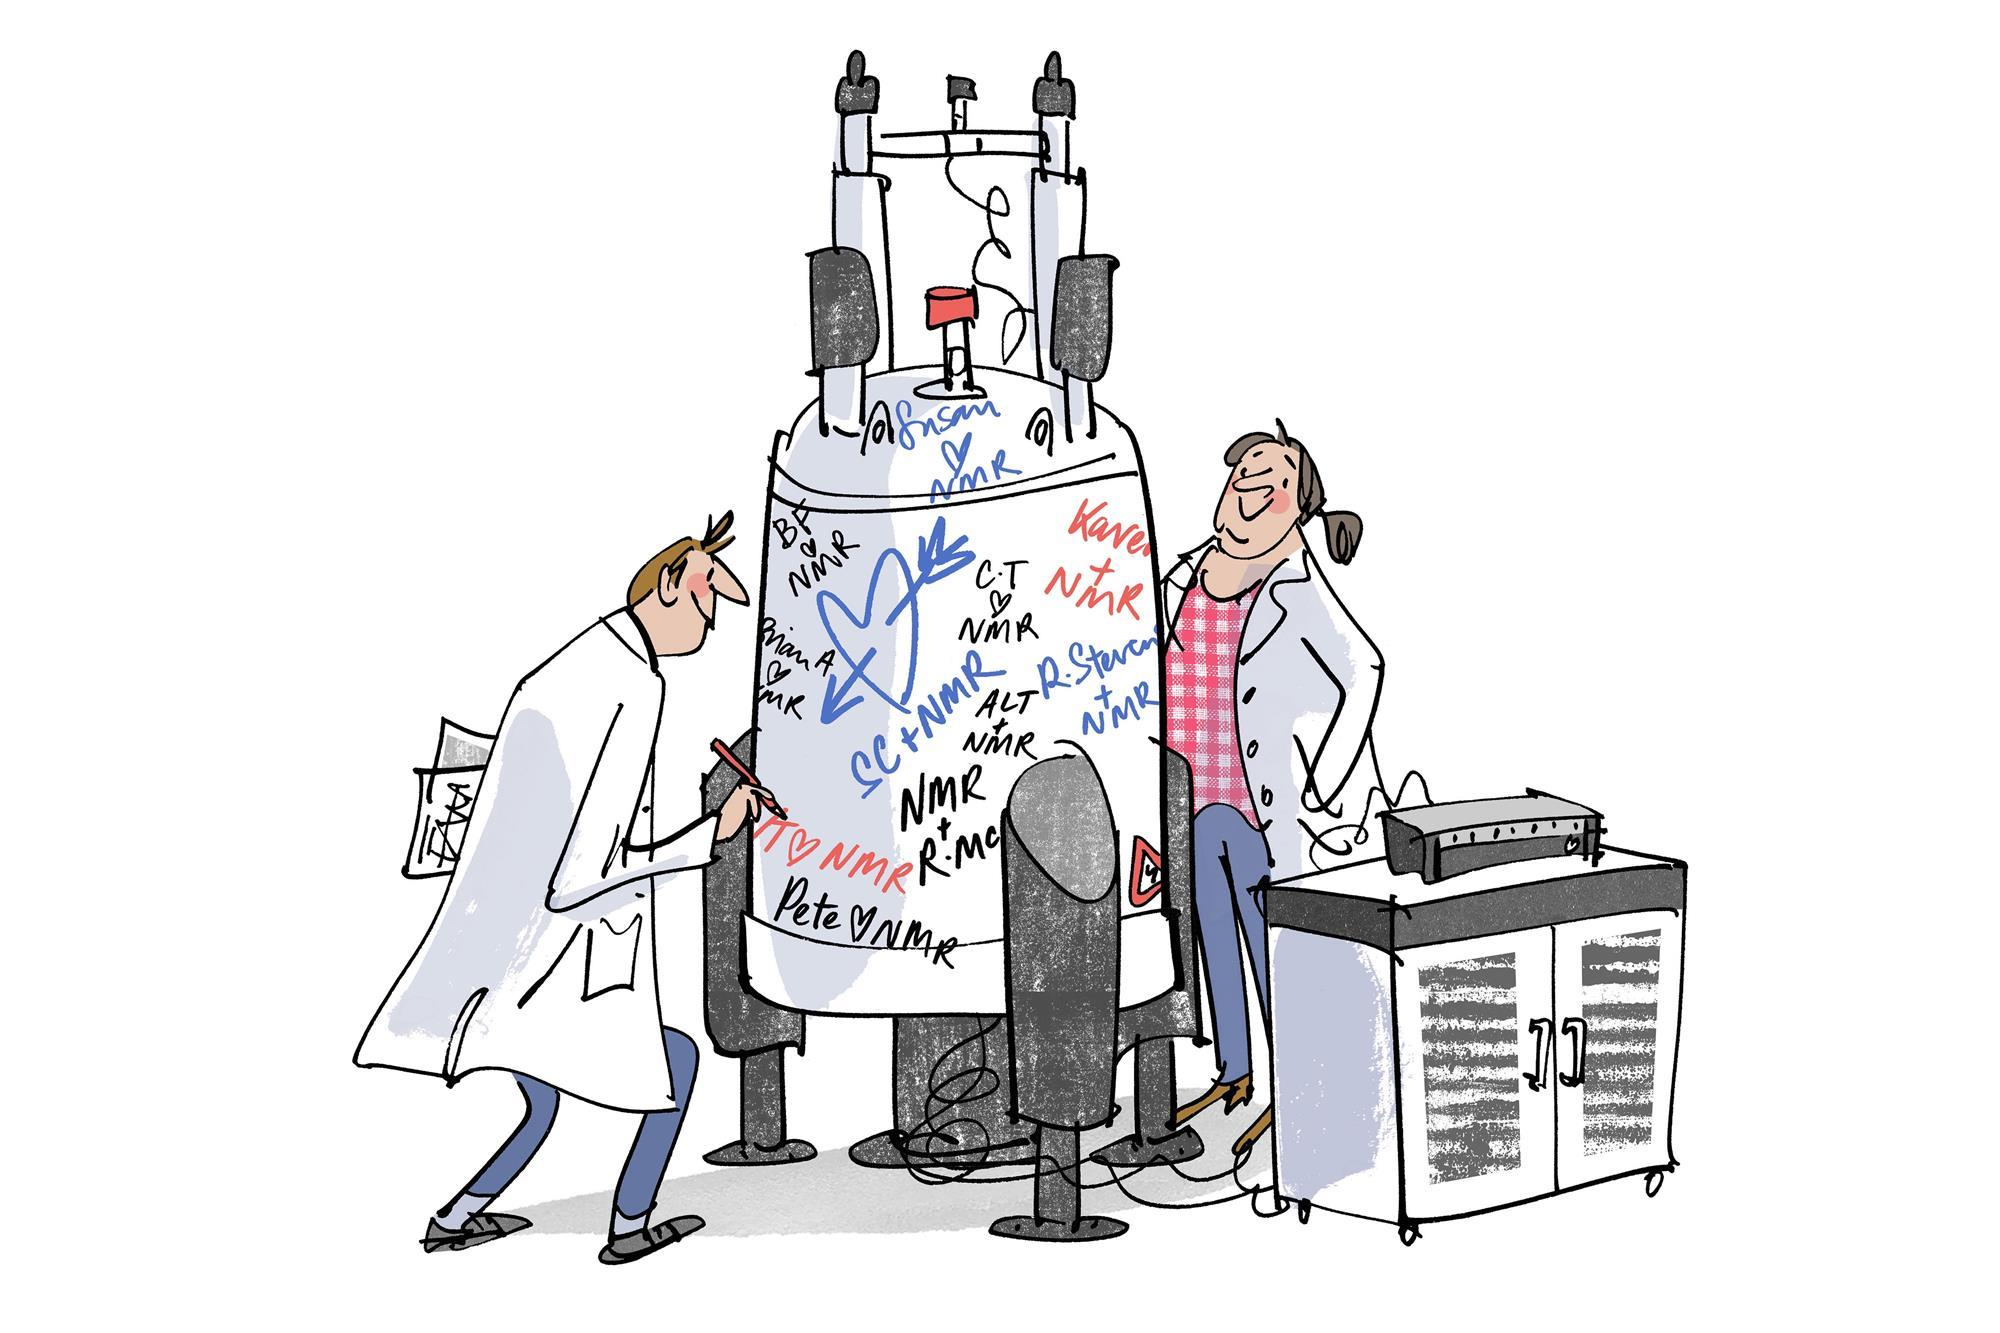
\includegraphics[height=4cm]{./images/cartoon.jpg}
    \end{center}
          \caption{\cite{cady_2020}}
    \label{fig:cartoon}
  \end{figure}
        \end{columns}
\end{frame}


\subsection{PNMR Techniques}
\begin{frame}
  \frametitle{Conventional MRI}
  % a comment
  \begin{figure}[htbp!]
    \begin{center}
      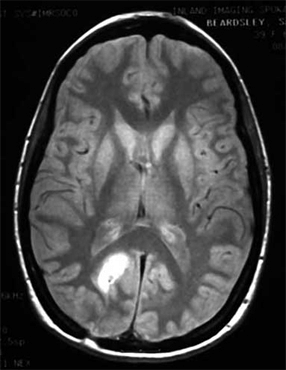
\includegraphics[height=6cm]{./images/mri_tumor.png}
    \end{center}
          \caption{MRI Scan of a Brain \cite{mri_tumor}}
    \label{fig:mri_tumor}
  \end{figure}
\end{frame}

\begin{frame}
  \frametitle{Conventional MRI}
  % a comment
  \begin{figure}[htbp!]
    \begin{center}
      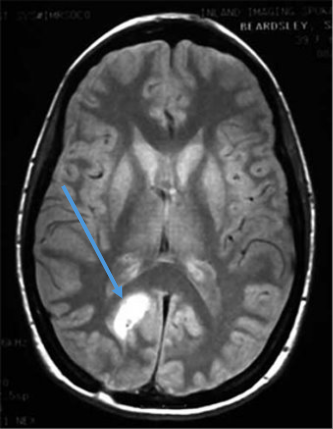
\includegraphics[height=6cm]{./images/mri_tumor_arrow.png}
    \end{center}
          \caption{MRI Scan of a Brain \cite{mri_tumor}}
    \label{fig:mri_tumor_arrow}
  \end{figure}
\end{frame}

\begin{frame}
  \frametitle{Metabolite Identification}
  % a comment
  \begin{figure}[htbp!]
    \begin{center}
      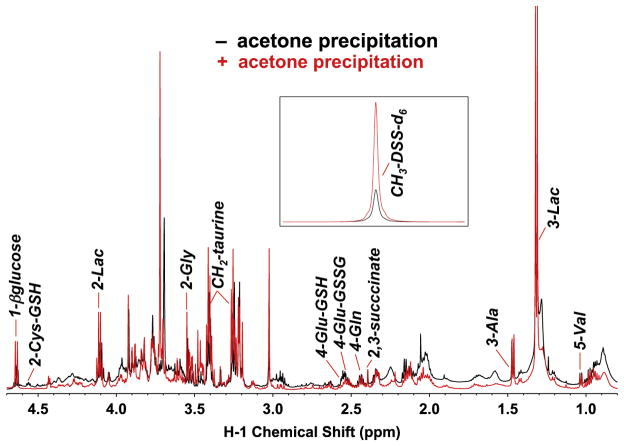
\includegraphics[height=6cm]{./images/chem_shift.jpg}
    \end{center}
          \caption{\cite{nmr_biochem}}
    \label{fig:chem_shift}
  \end{figure}
\end{frame}
\section{Methods}
\subsection{$180^{\circ}\,—\,90^{\circ}$}
\begin{frame}
  \frametitle{$180^{\circ}—90^{\circ}$ Pulses}
  % a comment
        \begin{center}
                \begin{figure}
                \begin{center}
                        
\includegraphics[height=3cm]{./images/cyclus.png}
                \end{center}
                \caption{}
                \label{fig:cyclus}
                \end{figure}
        \end{center}
\end{frame}

\section{Results}
\begin{frame}
  \frametitle{Transition Scenarios}
  % a comment
  \begin{columns}
    \column[t]{5cm}
    Scenario Details:
      \begin{itemize}
              \item SMR deployments begin in 2025
              \item Scenarios run from 1965 to 2090
              \item $UF_6$ processing capacity limits enrichment facilities
              \item All scenarios incorporate existing reactors, decommissioning on current timelines (e.g. Dresden generating station is active until 2029)
      \end{itemize}
    \column[t]{5cm}
  \begin{figure}[htbp!]
    \begin{center}
      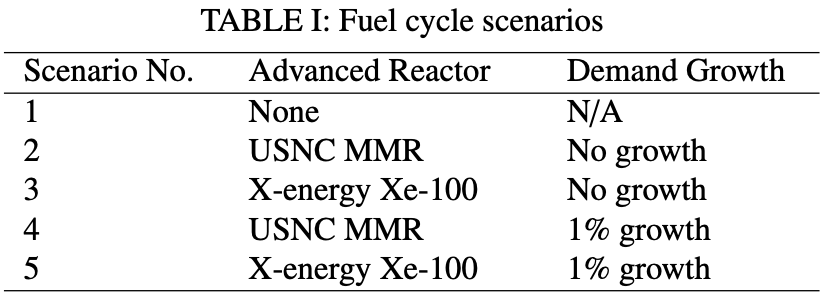
\includegraphics[height=2cm]{./images/scenarios.png}
    \end{center}
          \caption{}
    \label{fig:scenarios}
  \end{figure}
\end{columns}
\end{frame}

\section{Conclusion}
\subsection{Conclusion}
\begin{frame}
        \frametitle{Mass and SWU}
        % a comment
        \begin{columns}
                \column[t]{5cm}
                \begin{figure}
                        \begin{center}
                                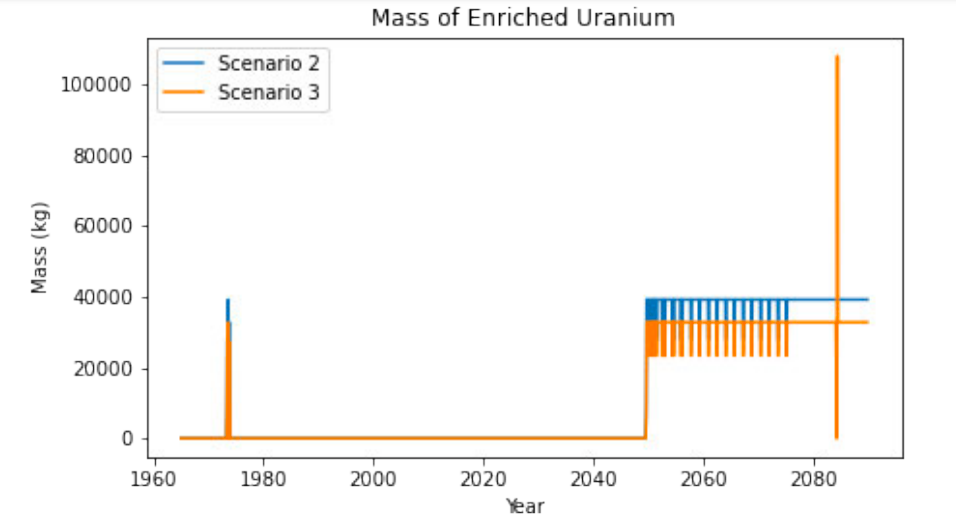
\includegraphics[height=2.7cm]{./images/mass.png}
                        \end{center}
                                \caption{Mass of Enriched Uranium.}
                        \label{fig:mass}
                \end{figure}
                \column[t]{5cm}
                \begin{figure}[htbp!]
                        \begin{center}
                                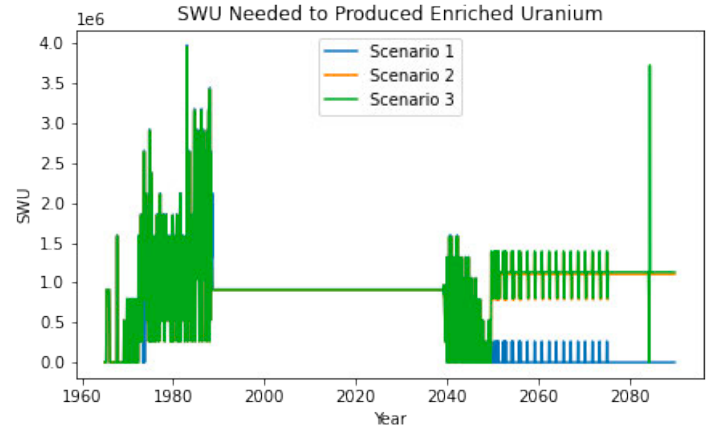
\includegraphics[height=3cm]{./images/swu.png}
                        \end{center}
                                \caption{Seperative Work Units needed for enrichment.}
                        \label{fig:swu}
                \end{figure}
              \end{columns}
\end{frame}


\begin{frame}
        \frametitle{Conclusions and Energy Use}
        % a comment
              \begin{columns}
                      \column[t]{5cm}
                        \begin{itemize}
                                \item Transition will require a mixture of HALEU production methods and deployments
                                \item Scenario 2 never reaches required power level
                                \item Scenario 3 requires more SWU than 2 due to higher enrichment
                        \end{itemize}
                      \column[t]{5cm}
              \begin{figure}[htbp!]
              \begin{center}
            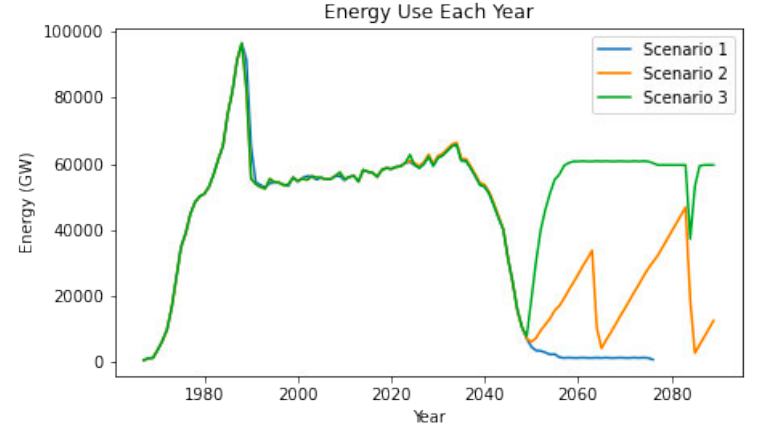
\includegraphics[height=3cm]{./images/e_use.png}
          \end{center}
                \caption{Energy use in each year. \cite{bachmann}}
          \label{fig:e_use}
        \end{figure}
              \end{columns}
\end{frame}

\subsection{Continuing Study}
\begin{frame}
    \frametitle{Further Analysis of Sample K}
    % a comment
    \begin{columns}
            \column[t]{5cm}
            \begin{figure}
                    \begin{center}
                            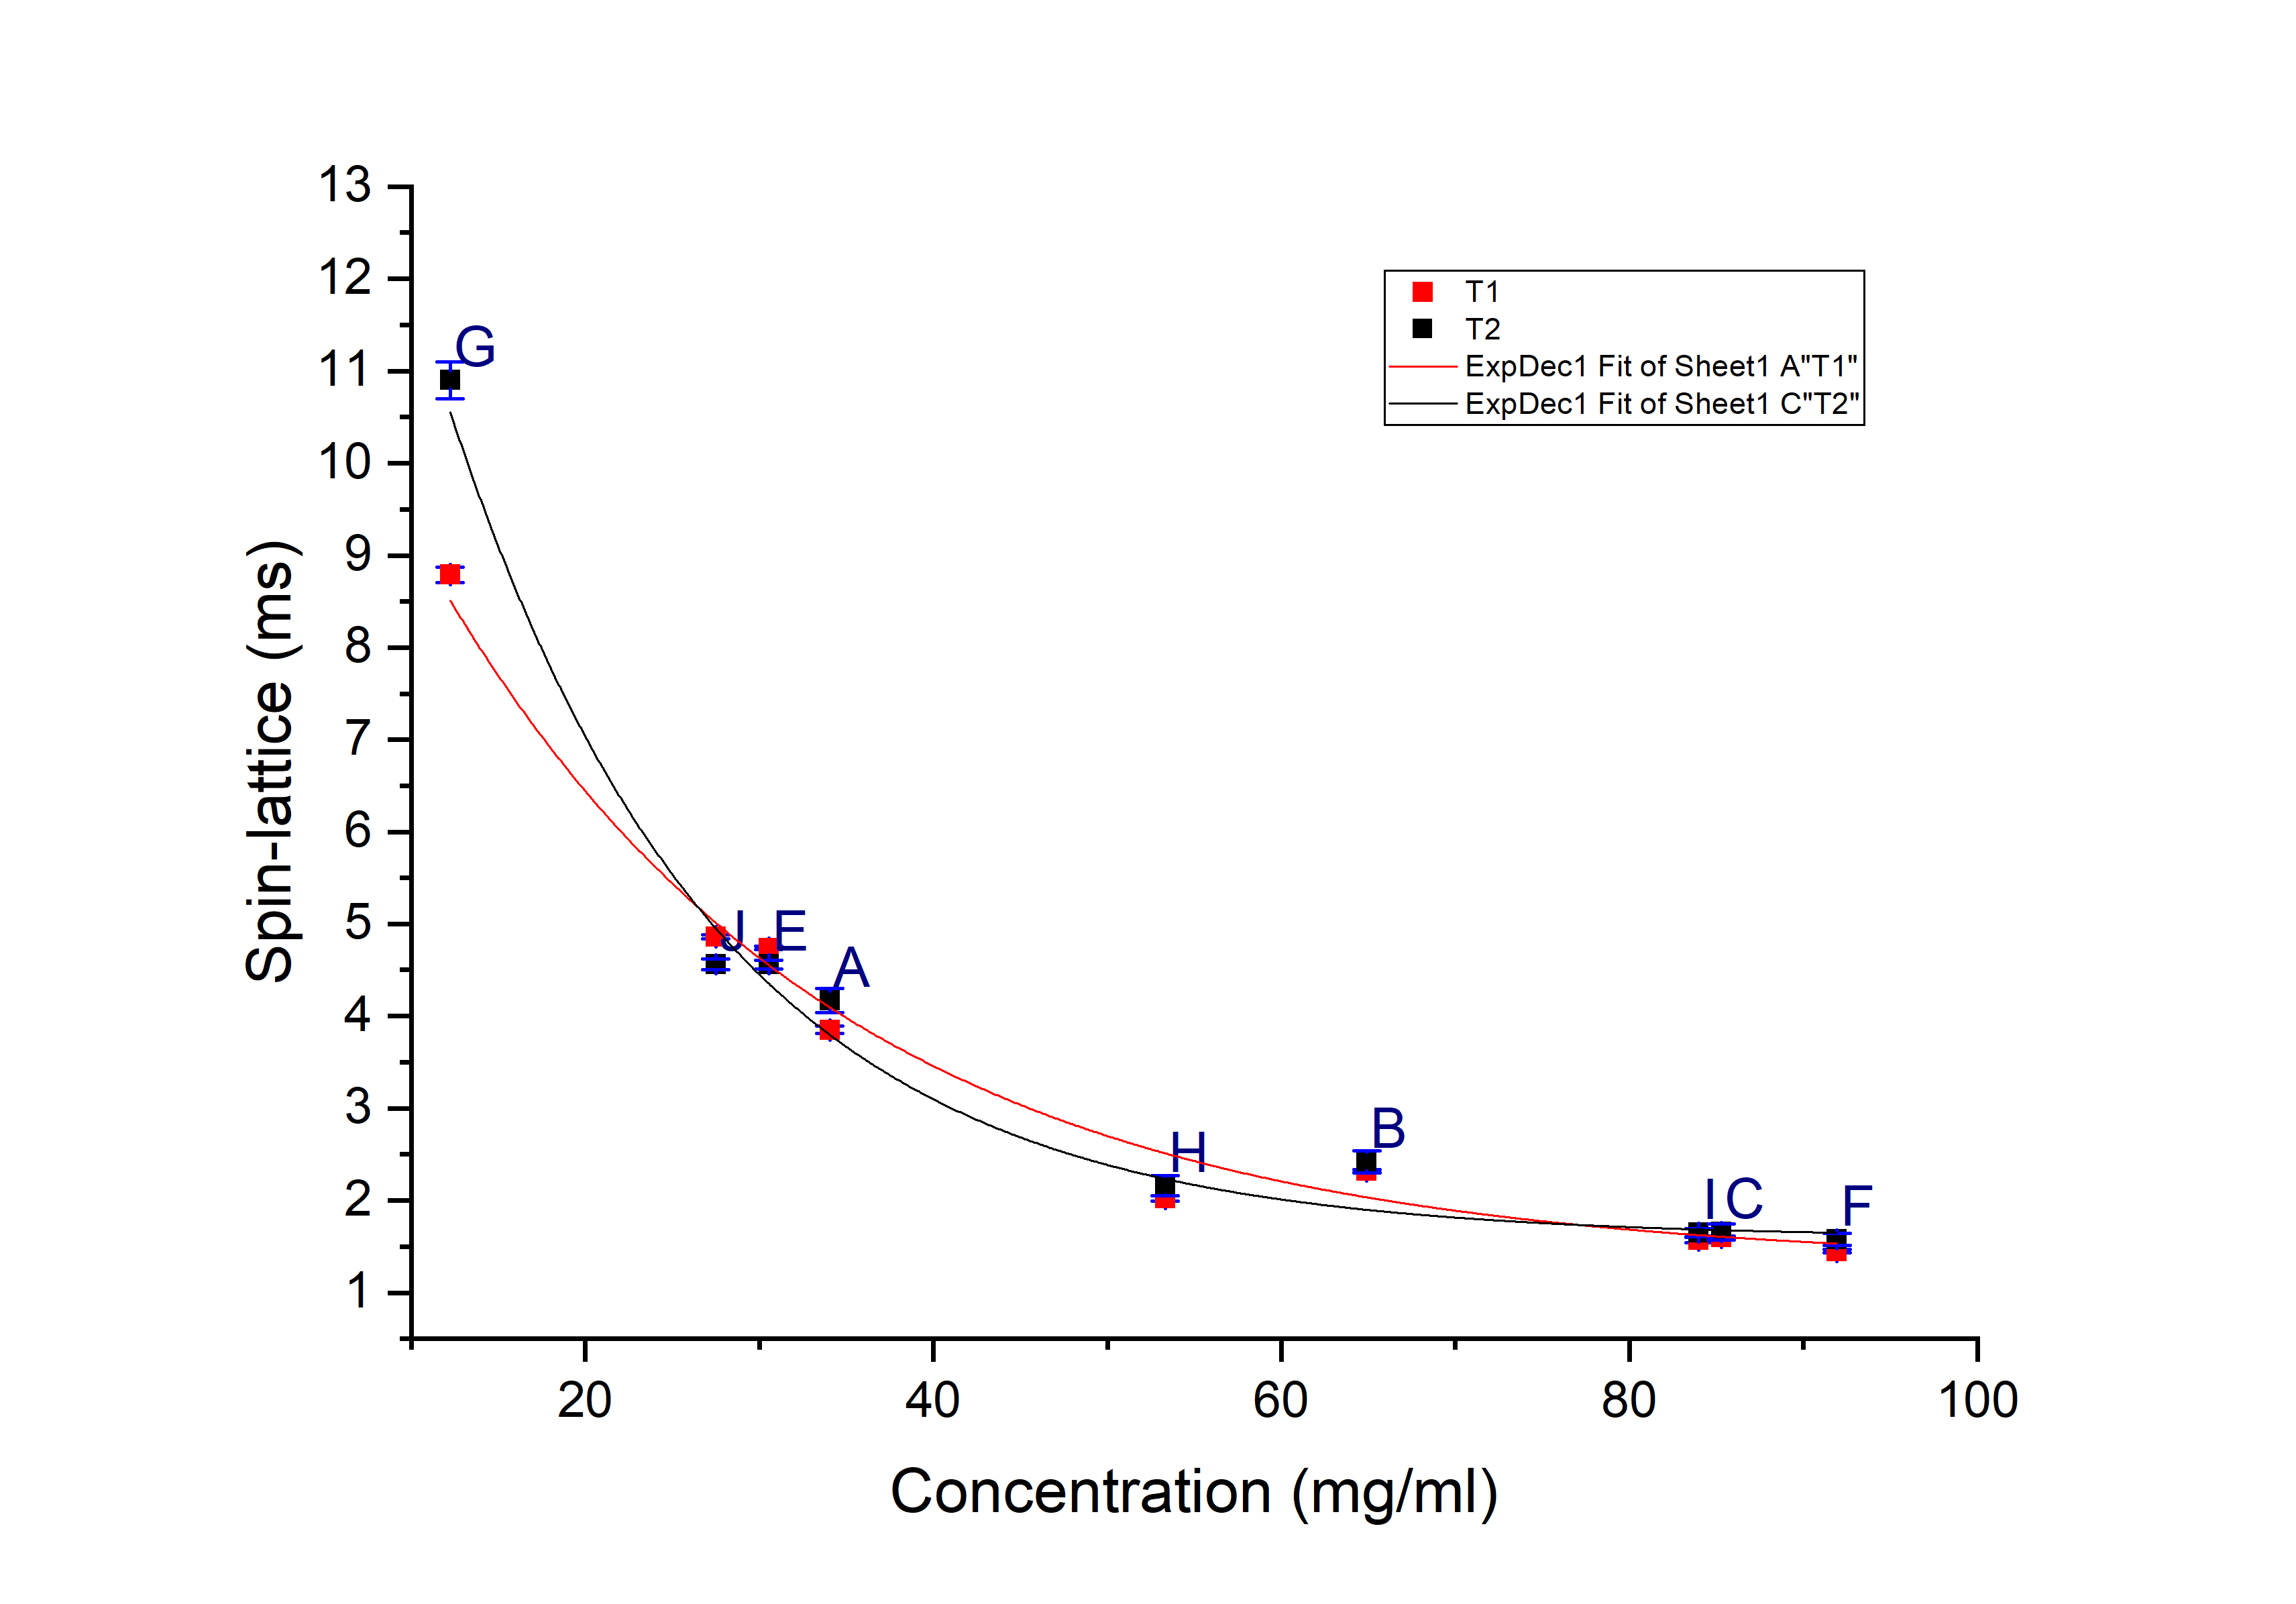
\includegraphics[scale=0.17]{./images/figures/res_k/res_w-out_k.jpg}
                    \end{center}
                            \caption{Fit without Sample K}
                    \label{fig:w-out_k}
            \end{figure}
            \column[t]{5cm}
                \begin{itemize}
                        \item The $T_1$ fit indicates a concentration of 37.9
                        \item The $T_2$ fit indicates a concentration of 33.4
                \end{itemize}
            Superficial literature review revealed no indication that this range of concentrations should behave differently.
          \end{columns}
\end{frame}

%%--------------------------------%%
%%--------------------------------%%
\begin{frame}[allowframebreaks]
  \frametitle{References}
  \bibliographystyle{plain}
  {\footnotesize \bibliography{bibliography.bib} }

\end{frame}
%%--------------------------------%%
\begin{frame}
  \frametitle{Acknowledgement}
        Acknowledgements should include both people who helped and funding 
        streams. If you are funded by an NEUP grant, that number usually goes 
        here. .
\end{frame}

\input{end}
\begin{frame}
    \frametitle{Relaxation Path}
    % a comment
    \begin{figure}[htbp!]
      \begin{center}
        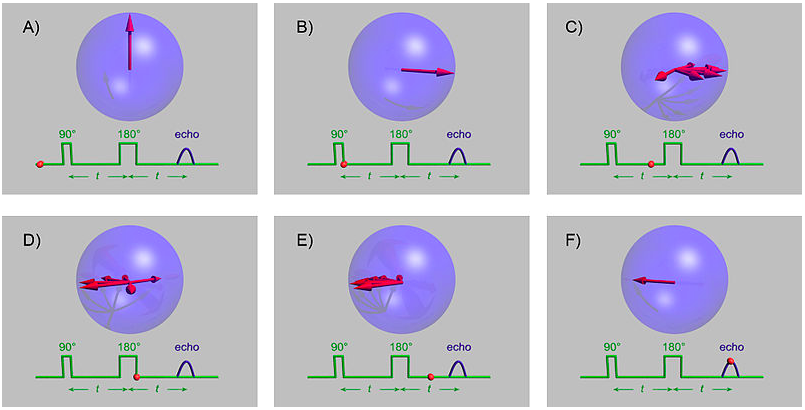
\includegraphics[width=\linewidth]{./images/figures/theory/relax.png}
      \end{center}
            \caption{General Relaxation Path \cite{spin_echo}}
      \label{fig:relax}
    \end{figure}
  \end{frame}

\begin{frame}
    \frametitle{Frequency Deviation}
    % Talk about the wacky result from sample D around 0.17, what's doing 
    \begin{figure}[htbp!]
        \begin{center}
            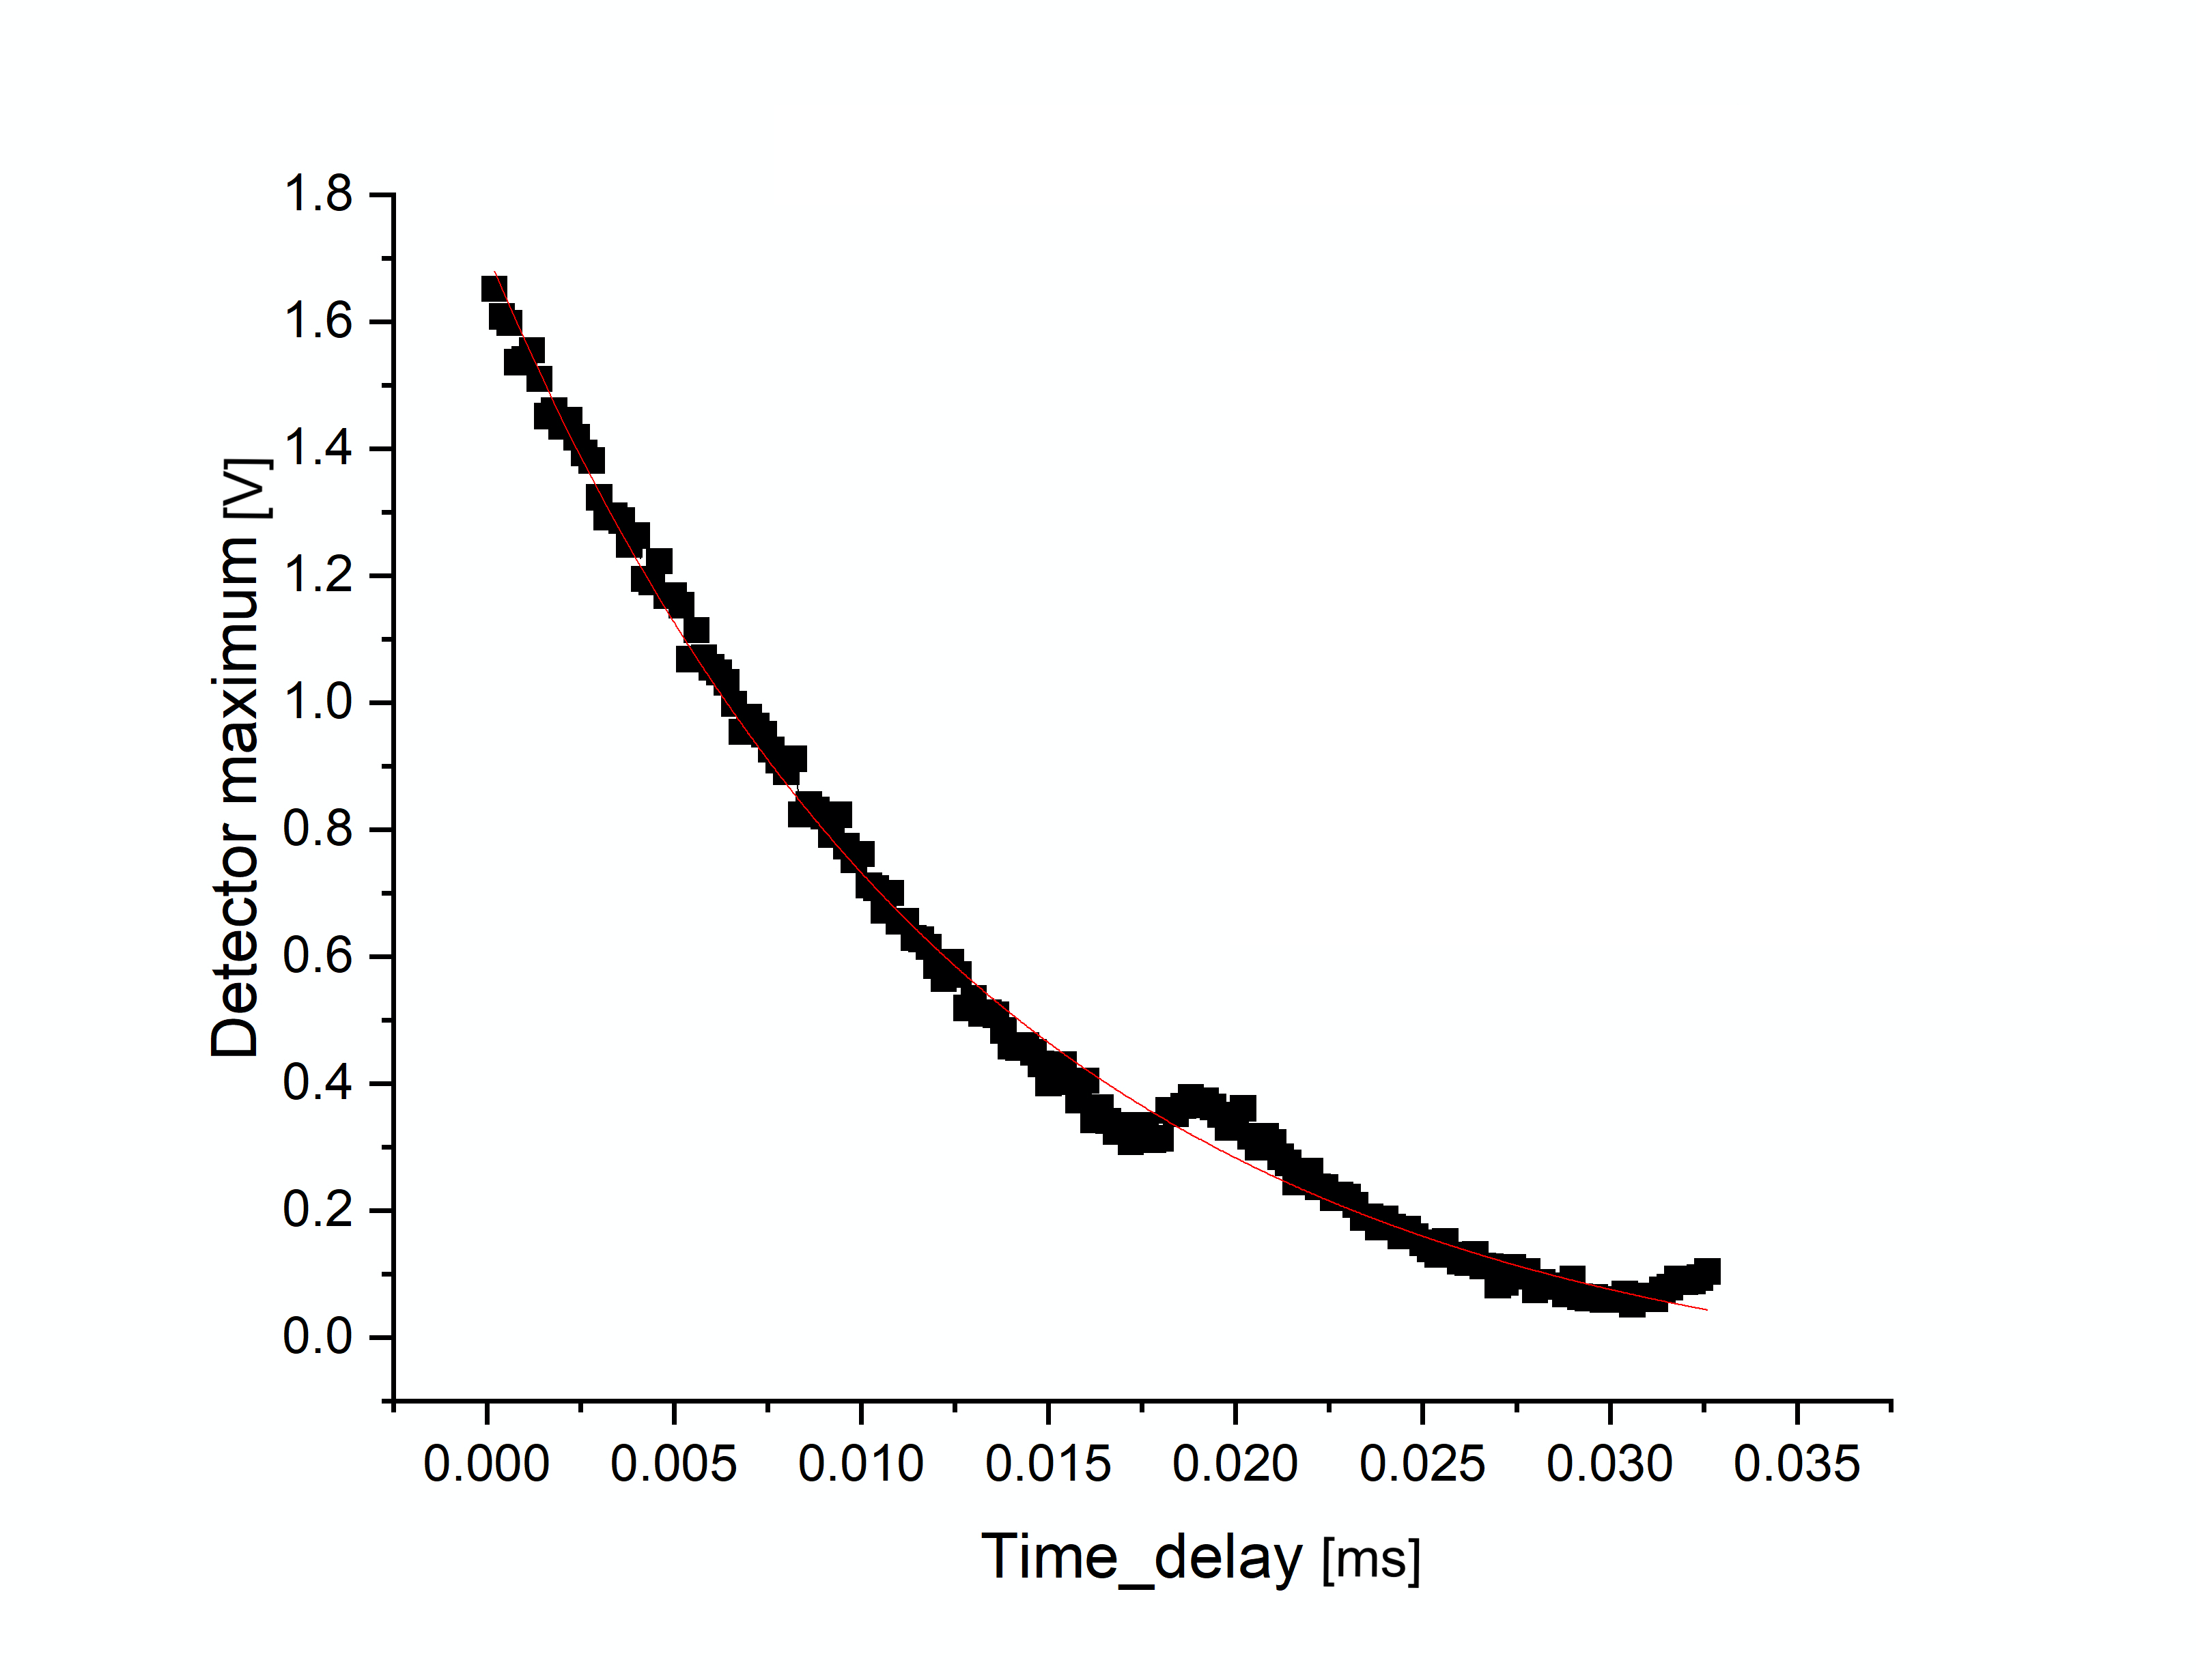
\includegraphics[scale=0.31]{./images/figures/theory/d-t1.png}
        \end{center}
                \caption{Sample D [$ 3.37 \pm 1.6 x 10^{-2}$]:$ T_1$}
        \label{fig:d_t1}
    \end{figure}
\end{frame}

\begin{frame}
    \frametitle{Exceeding Relaxation Time}
    \begin{figure}[htbp!]
        \begin{center}
            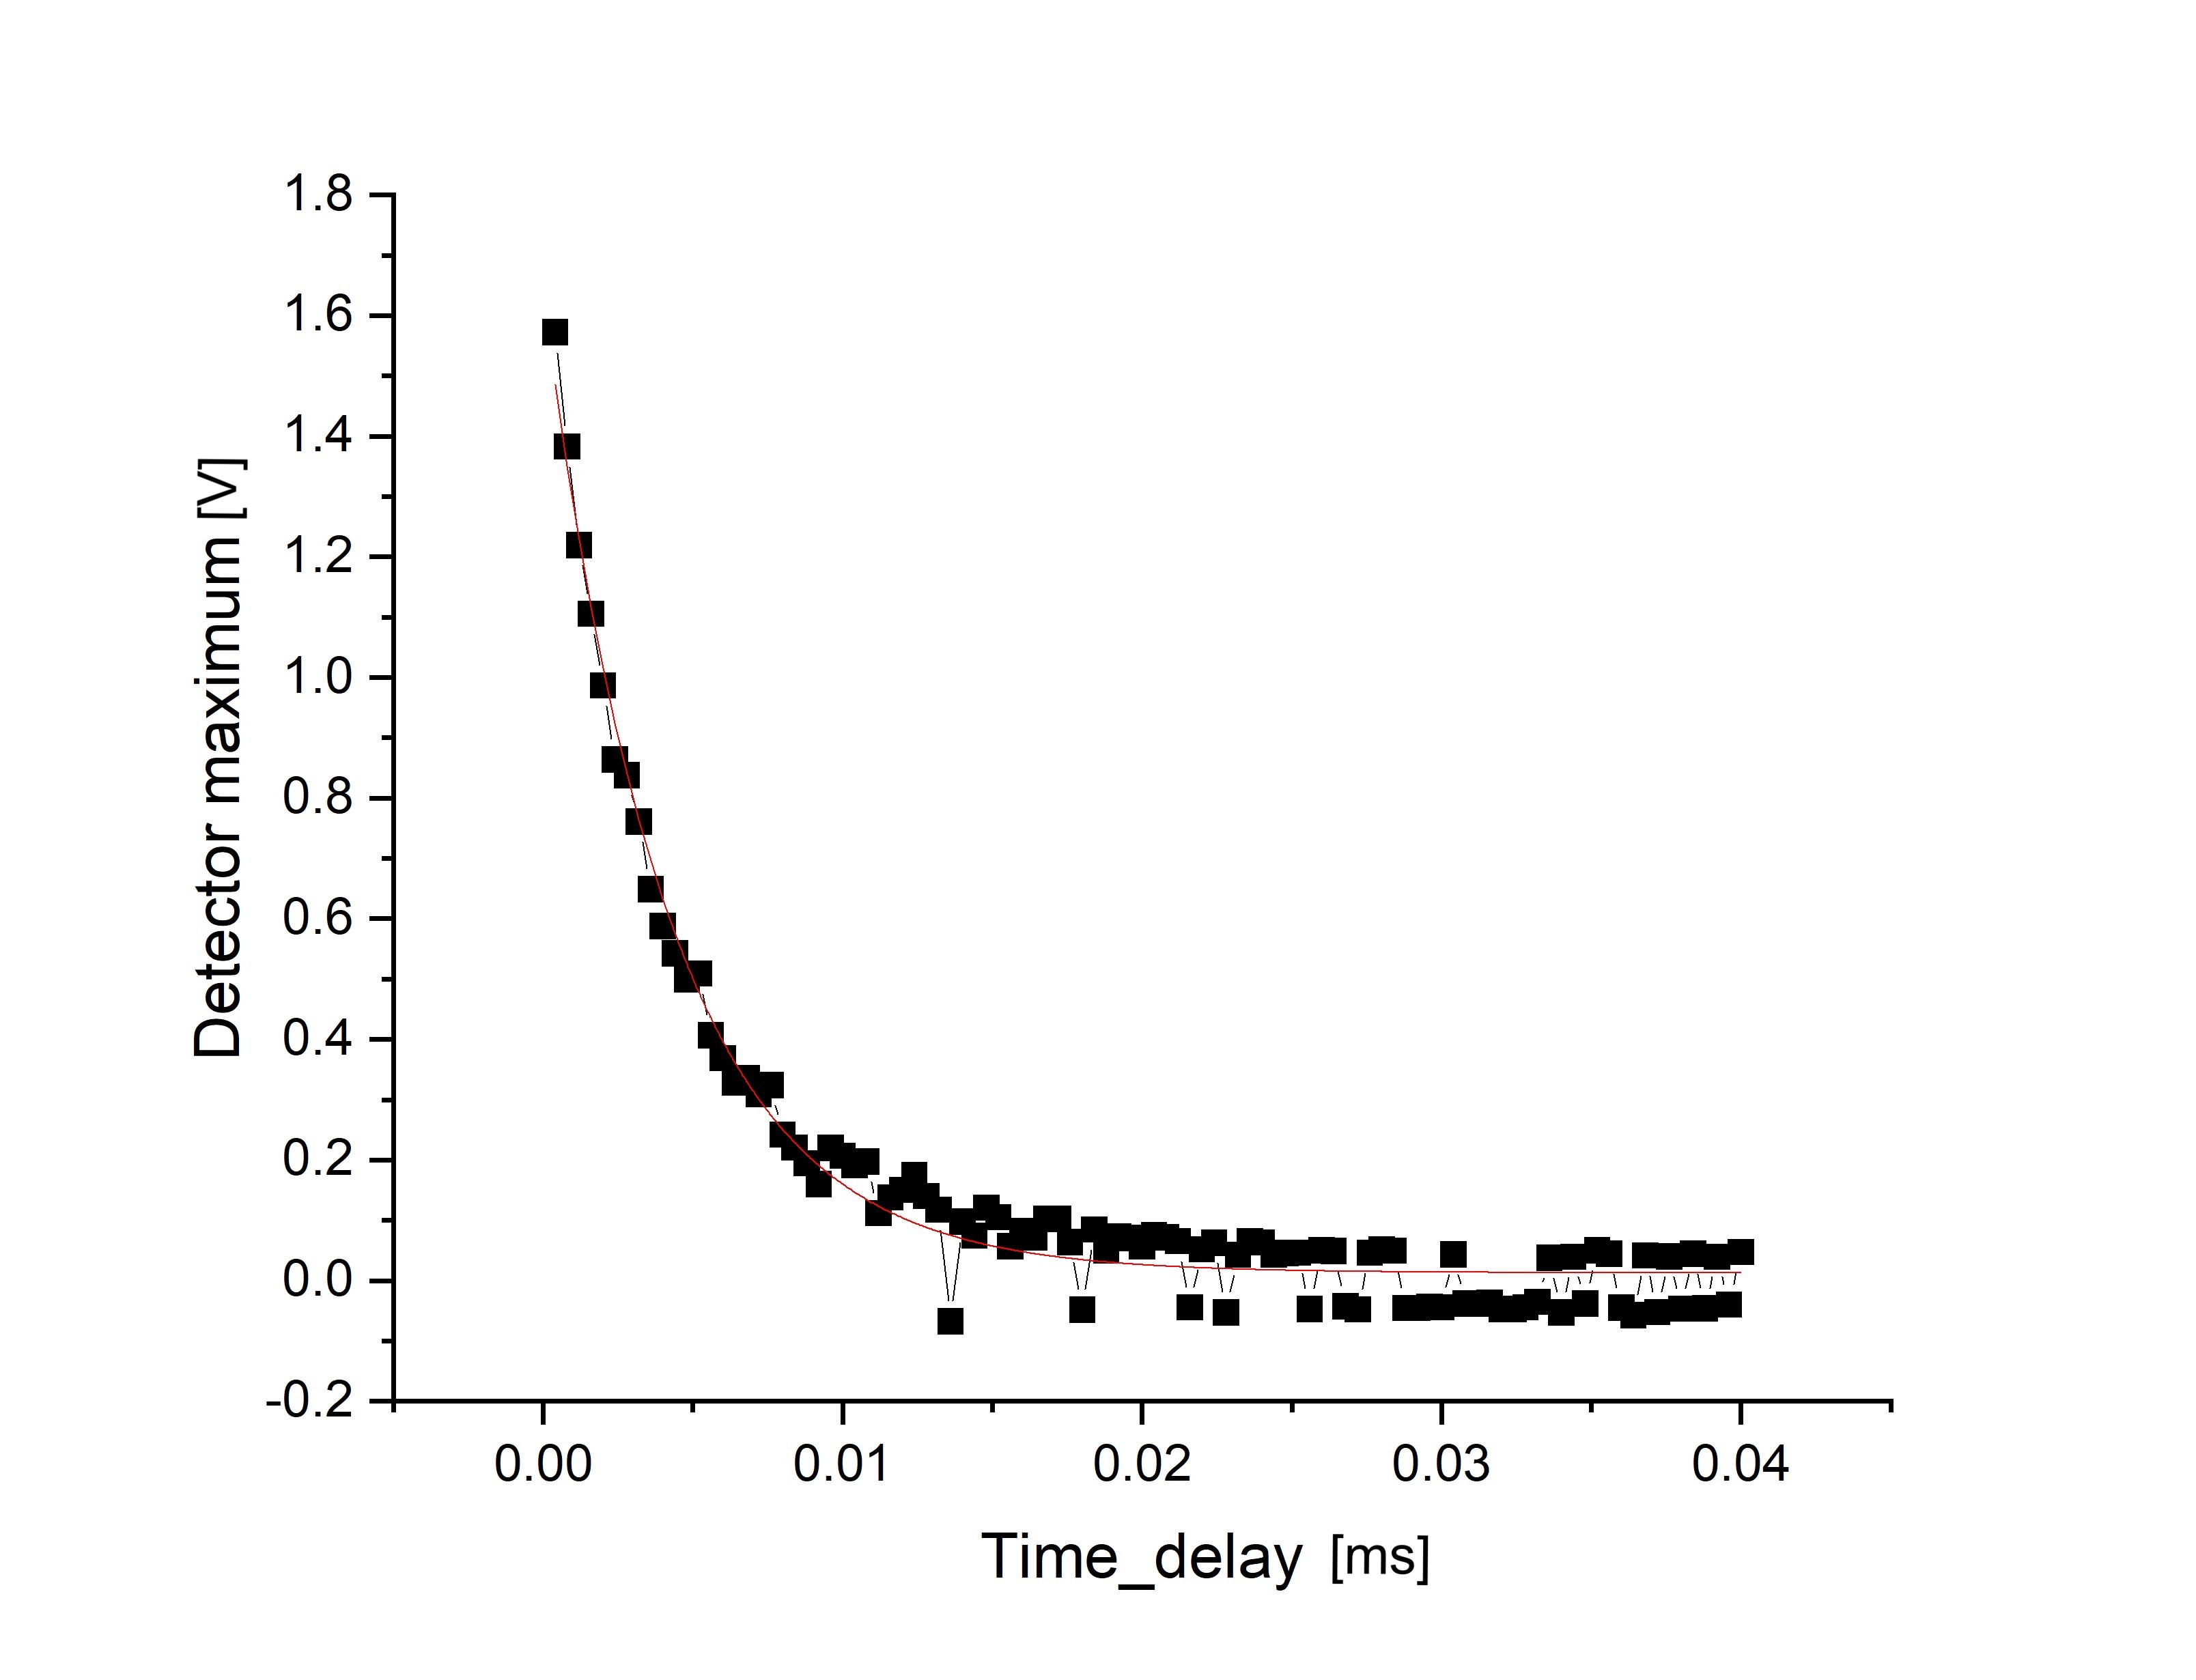
\includegraphics[scale=0.07]{./images/figures/t_plots_appendix/a_t-2.jpg}
        \end{center}
                \caption{Sample A [$ 34.0 \pm 6.0 x 10^{-2}$]:$ T_2$}
        \label{fig:a_t2}
    \end{figure}
\end{frame}

\end{document}



